\chapter{Adaptive Informationsverteilung mit RSS und verteiltem Publish/Subscribe}
Im Folgenden beschreiben  wir eine Methode, ereignisbasierte Informationen an interessierte Klienten zu verteilen. Wir orientieren
uns dabei an RSS. Mit ``Ereignis'' meinen wir im Folgenden eine Informationseinheit (z. B. eine Nachrichten-Schlagzeile),
mehrere Ereignisse k�nnen in einem Datenpaket (RSS-Feed) gesammelt an den Klienten �bermittelt werden. Dazu betrachten wir zun�chst, nach welchem
Schema die Informationen entsprechend dem RSS-System verbreitet werden, zeigen daraus resultierende Probleme auf und schlagen ein Konzept vor,
wie diese Probleme vermieden bzw. verringert werden k�nnen. Auch wenn wir im Folgenden �berwiegend von RSS sprechen, so l�sst sich das Konzept auch auf
andere Informationssysteme �bertragen, die bestimmte Kriterien erf�llen. Je nachdem, auf welche Ebene wir uns beziehen, werden wir entweder von ``Informationen''
oder ``RSS-Feeds'' sprechen. Das neu entwickelte System wollen wir im Folgenden ``\pubsubrss'' nennen.
 
\section{Verteiltes Polling}
Betrachten wir die Gesamtheit der Subscriber und ihr Polling-Verhalten, so erkennen wir, dass aus Sicht eines RSS-Servers die Polling-Frequenz
dieser Gesamtheit (mittlere Ankunftsrate der Anfragen) gr��er ist als die Polling-Frequenz jedes einzelnen Subscribers.
W�nschenswert w�re es, wenn jeder Subscriber von der
Polling-Frequenz der Gesamtheit profitieren k�nnte, so dass die gesteigerte Frequenz zu einer erh�hten Aktualit�t der RSS-Feeds beim entsprechenden
Subscriber f�hrt. Es bietet sich an, die Subscriber �ber ein Overlay-Netzwerk zu verbinden, so dass die RSS-Feeds zwischen den Subscribern ausgetauscht werden
k�nnen. Das Polling wird also auf die beteiligten Subscriber verteilt.
Wir haben es dabei mit einer Kombination aus einem Pull- und einem Push-Ansatz zu tun. Allerdings �bernimmt die Push-Funktion nicht der RSS-Server,
sondern sie wird von den beteiligten Einheiten des Overlay-Netzes �bernommen, von dem der RSS-Server kein Bestandteil ist. Es stellt sich die Frage,
warum wir nicht gleich den Push-Ansatz bezogen auf den RSS-Server favorisieren. RSS ist eine schon seit l�ngerer Zeit bestehende Technik.
Dar�ber hinaus ist RSS weit verbreitet.
Eine Modifikation des Grundkonzeptes w�rde f�r Anbieter, die es unterst�tzen, bedeuten, bestehende Software austauschen zu m�ssen und
ganz neue Serviceleistungen bereitstellen zu m�ssen. Dies w�rde m�glicherweise auf Ablehnung sto�en und damit nicht die gew�nschte
Verbreitung des neuen Konzeptes mit sich bringen. Ziel ist es, auf dem bestehenden Konzept aufzubauen und es in ein erweitertes Konzept zu
integrieren, um f�r den Benutzer als auch f�r den Dienstanbieter m�glichst ein Minimum an Aufwand zu erreichen (Deolasee et al.
besch�ftigen sich in \cite{bhide02adaptive} mit einer Kombination aus Push-Pull und beschreiben die Probleme, die sich aus reinen Pull- bzw.
Push-Ans�tzen ergeben).
\subsubsection*{Einbettung in PubSub}
Es ist naheliegend, das Publish-Subscribe-Kommunikationsparadigma auf unser Problem anzuwenden: Die Informationen, konkret also die RSS-Feeds, sollen �ber ein
Notifikationssystem an die Interessenten (Subscriber) ausgeliefert werden. Da sich die Funktion bzw. Rolle des RSS-Servers nicht �ndern
soll, muss die Funktion des Publishers eine andere Einheit �bernehmen. Es bietet sich an, die Rolle des Publishers ebenfalls den Klienten
zuzuweisen. Ein Klient erh�lt in der Rolle des Subscribers nach einer Anfrage seinerseits den RSS-Feed von einem RSS-Server.
Der Klient kann nun diesen Feed in
der Rolle des Publishers in das Notifikationssystem einspeisen. Das Notifikationssystem soll aus einem System von vernetzten Brokern
bestehen. Ein Broker, welcher einen Feed erh�lt, liefert diesen an die �brigen mit ihm verbundenen Subscriber bzw. Broker aus. F�r einen
Subscriber gibt es also zwei M�glichkeiten, einen Feed zu erhalten: entweder auf direkte Anfrage von einem RSS-Server (Pull) oder �ber
das Notifikationssystem (Push). Um einen neuen Feed zu erhalten, kann ein Subscriber selbst aktiv werden und den Feed vom RSS-Server anfordern, oder er kann warten,
bis ihm ein neuer Feed durch das Netzwerk �ber einen Broker �bermittelt wird. Es ergeben sich dabei folgende Fragestellungen: wann soll ein
Klient aktiv werden, um den RSS-Server zu kontaktieren, und wann soll ein Klient inaktiv bleiben, um den Feed �ber das Brokernetzwerk zu erhalten? Denn
folgende Problemsituation ist denkbar: kontaktieren alle Klienten gleichzeitig den entsprechenden RSS-Server, so bringt dies keine Vorteile, da dies dem alten Ansatz
entspricht; erreicht der neue Feed
einen Klienten �ber einen Broker, so besitzt der Klient diesen neuen Feed bereits, da er zuvor eigenm�chtig den RSS-Server kontaktiert hat.
\todo{Filter}
\subsubsection*{Ansatz: Ein Publisher}
Die einfachste L�sung w�re, einen dedizierten Publisher zu bestimmen, welcher als alleiniger Klient das Polling �bernimmt. Alle weiteren Klienten
w�rden die Feeds �ber das Broker-Netzwerk erhalten. Vorteil w�re, da� es relativ wenig
Anfragen an den RSS-Server g�be. Die Nachteile �berwiegen jedoch: in Abh�ngigkeit von der Netzstruktur kann es zu langen �bertragungszeiten der Feeds f�r einzelne
oder mehrere Subscriber kommen. Wir m�ssten eine geringere Aktualit�t der Daten \todo{in Kauf} nehmen. Zudem h�tten \todo{}wir das Problem des
\glqq Single Point of Failure\grqq: f�llt der dedizierte Publisher aus, kann die Verbreitung der Feeds zun�chst nicht mehr erfolgen.
Erst, nachdem das Netzwerk den Ausfall registriert hat und entsprechende Gegenma�nahmen eingeleitet hat (z. B. Bestimmung eines neuen dedizierten
Publishers), kann es zu einer weiteren Verbreitung der Feeds kommen. Dar�ber hinaus k�nnten die Klienten nicht von verteiltem Polling profitieren.
\subsubsection*{Ansatz: Mehrere Publisher}
Daher favorisieren wir eine L�sung, bei der zu gegebener Zeit nur eine gewisse Auswahl der Klienten gleichzeitig Anfragen an den RSS-Server senden.
Es muss also zu einer Abstimmung bzw. Koordinierung der Klienten untereinander kommen, um diese Auswahl zu bestimmen. Auch hierbei ist zu beachten,
dass Ausf�lle von Publishern im Netz nicht zu Datenverlust f�hren sollen; d. h. jeder Subscriber sollte die Informationen bzw. Feeds, die er zu erhalten w�nscht,
auch dann erhalten, wenn die f�r das Polling vorgesehenen Klienten ausfallen.


\section{Rolle der Broker}
Broker sind der zentrale Bestandteil des Notifikationssystems. Das Notifikationssystem besteht aus einer Reihe von Brokern,
die untereinander verbunden sind und ein zusammenh�ngendes Netz bilden (Overlay-Broker-Netzwerk, siehe dazu \cite{PietzuchBacon:2003:P2POverlay}).
Ein Broker empf�ngt Feeds von Brokern oder von Klienten/Publishern. Anschlie�end sorgt er f�r eine Verteilung der
Feeds an eine bestimmte Auswahl von mit ihm verbundenen Brokern bzw. Subscribern. Ein Broker kann also eine zentrale Sammelstelle f�r Feeds
unterschiedlicher Anbieter sein. Die einzelnen in den Feeds zusammengefassten Ereignisse k�nnen durch den Broker neu zusammengestellt werden.
Als Kriterien f�r neue Zusammenstellungen bieten sich die Aktualit�t der einzelnen Ereignisse sowie definierbare Filterregeln an. Einzelne 
Ereignisse, die den Broker bereits erreicht haben, brauchen nicht erneut weitergeleitet zu werden und finden daher nach unserem Konzept keinen
Eingang in die neu zusammengestellten Feeds. Dadurch k�nnen Netzressourcen gespart werden. Voraussetzung daf�r ist, dass der Broker einen Cache
unterh�lt, in dem Ereignisse zwischengespeichert werden.\\

Filter k�nnen durch Subscriber definiert und bei Brokern
hinterlegt werden. Aufgrund der Filterregeln k�nnen Ereignisse verschiedener
Anbieter aus den Feeds extrahiert und in einem neuen Feed gesammelt werden. Ein
Subscriber kann also eine individuelle Zusammenstellung der Ereignisse erhalten. Filterregeln und ihre Anwendung wurden schon ausf�hrlich
erforscht und sollen nicht Gegenstand dieser Arbeit sein. Deshalb fanden sie auch keinen Eingang in die weiter unten beschriebene
Simulationsumgebung. Sie erweitern die M�glichkeiten des Systems lediglich, haben aber keinen Einfluss auf das Grundkonzept, um das es hier geht.
Unser System \pubsubrss k�nnte mit bestehenden Pub/Sub-Systemen, welche Filtertechniken unterst�tzen (wie z. B. das System
REBECA \cite{MuFiBu:2001:ArchFrameECommApp}), kombiniert werden.\\

Der folgende Absatz beschreibt Vorg�nge, die eigentlich Teil des jeweiligen Notifikationsdienstes sind, von dem wir abstrahieren. Da jedoch ein
spezifisches Verhalten des Notifikationsdienstes auf eine optimale Funktionsweise des Systems Einfluss nehmen kann, werden wir einige Vorg�nge beschreiben.\\ 

Um sich dem entsprechenden Broker bekannt zu machen und Filter zu hinterlegen, muss sich ein Subscriber bei diesem Broker mit einer speziellen
Registrierungsnachricht registrieren.
Ein Broker braucht nur an diejenigen Subscriber aktuelle Feeds zu �bermitteln, welche auch tats�chlich online sind. Zus�tzlich ist es also notwendig,
dass ein Subscriber in regelm��igen Zeitabst�nden den jeweiligen Broker �ber seinen Online-Status unterrichtet (nennen wir eine solche Nachricht
\glqq KEEPALIVE-Nachricht\grqq{}). Erh�lt ein Broker eine KEEPALIVE-Nachricht eines Subscribers, f�r den er den Zustand \glqq ist offline\grqq{} gespeichert hat,
sollte er diesem eine Zusammenstellung der aktuellsten Ereignisse �bermitteln. Denn kommt es aufgrund von St�rungen im physischen Netzwerk oder
aufgrund von Netz�berlastung zu verloren gegangenen KEEPALIVE-Nachrichten, so gilt der Subscriber f�r seinen Broker als \glqq offline\grqq{}. Dieser wird ihm
daraufhin keine Feeds mehr �bermitteln.\\
Hat der Subscriber aufgrund von adaptiven Ma�nahmen seine aktuelle Polling-Periode stark angehoben, so wird er zun�chst keine weiteren Feeds beim
entsprechenden RSS-Server selbst�ndig erfragen, so dass ihm eventuell Informationen verloren gehen. Die Menge verloren gegangener Informationen
kann geringer gehalten werden, wenn dem Subscriber die letzten Ereignisse bei Wiedereintritt in das Overlay-Netzwerk als Feed �bermittelt werden.
Entsprechend sollte ein Subscriber seinen jeweiligen Broker dar�ber informieren, wenn er offline geht, um unn�tigen Datentransfer zu vermeiden.\\

Im Zusammenhang mit Brokern werden noch einige weitere Ma�nahmen und Nachrichtentypen notwendig sein, auf die wir jedoch erst in sp�teren Kapiteln zu sprechen
kommen werden, da sie Anpassungen an spezielle Bed�rfnisse darstellen (siehe Kapitel \glqq Churn\grqq{} \ref{cs:churn}) .
%%% Local Variables: 
%%% mode: latex
%%% TeX-master: "diplomarbeit"
%%% End: 

\section{Koordinierung der Subscriber}

Um das Netz nicht noch zus�tzlich zu belasten, sollte die Netzbelastung, die durch eventuelle Abstimmungsnachrichten entsteht, minimal sein.
Die Konzeption eines Algorithmus sollte unter folgenden Gesichtspunkten erfolgen:
\begin{itemize}
  \item Polling durch mehrere bzw. wechselnde Klienten
  \item Anfragen an den RSS-Server sollten nicht gleichzeitig f�r alle Klienten geschehen 
  \item Ausfall von Klienten im Overlay-Netzwerk soll Informationsverteilung nicht blockieren
  \item Netzbelastung durch Abstimmungsnachrichten sollte gering gehalten werden
\end{itemize} 
Im Folgenden beschreiben wir einen Algorithmus bzw. eine Technik, die unsere bisher gestellten Anforderungen erf�llt.
\subsection{Der Grundlegende Algorithmus}
\label{cs:der_grundlegende_algorithmus}
Es sei $t_0$ immer der aktuelle Zeitpunkt. Ausgehend von einem beliebigen Zeitpunkt
$t_x$ mit $t_0\leq t_x$ und einer Intervallspanne $\Delta Z$ w�hlt sich jeder
Subscriber $i$ innerhalb des Zufallsintervalls $Z:=[t_x,t_x+\Delta Z]$ einen zuf�lligen Zeitpunkt $ttr_i$ (``time to tefresh'', $ttr$ im allgemeinen), zu dem
er den aktuellen Feed vom RSS-Server erfragt (siehe Abb. \ref{Abb:determine_ttr}). Im Folgenden nennen wir $t_x$ Einstiegspunkt und $\Delta Z$ Zufallsspanne.

\begin{picturehere}{3}{1.5}{$ttr$s}{Abb:determine_ttr}
 
%\psset{xunit=1cm,yunit=1cm,runit=1cm}
%\begin{picture}(1.5,-0.5)(7,1)
\begin{picture}(7,1)(1.5,-0.5)
  \put(0,0){\vector(1,0){7}}
  \put(0,-0.2){\line(0,1){0.4}}
  \put(0,-0.5){$t_0$}
  \put(3,-0.2){\line(0,1){0.4}}
  \put(3,-0.5){$t_x$}
  \put(6,-0.2){\line(0,1){0.4}}
  \put(6,-0.5){$t_x+\Delta Z$}
  \put(5,-0.1){\line(0,1){0.2}}
  \put(4.5,0.4){$ttr_i$}
  \put(7.8,0){$time$}
\end{picture}
% \includegraphics{determine_ttr}
\end{picturehere}


Ist $ttr_i$ erreicht, so erfragt Subscriber $i$ den aktuellen Feed vom RSS-Server und setzt nun $ttr_i$ auf einen
Zufallswert innerhalb des
Zeitintervalls $Z:=[t_x,t_x+\Delta Z]$, wobei $t_x$ ebenfalls neu gew�hlt wird.
Erh�lt Subscriber $i$ vor dem Erreichen des Zeitpunktes $ttr_i$ einen Feed $feed_{new}$ von einem Broker zum 
Zeitpunkt $t_f$ (sei $feed_{old}$ der bisher bei $i$ gespeicherte Feed), so geschieht folgendes:
\pagebreak[3]
\begin{description}[\compact]
  \item [Fall I:] $feed_{new}$ ist nicht aktueller als $feed_{old}$:
    \begin{description}[\breaklabel\compact]
      \item keine �nderungen
    \end{description}
  \item[Fall II:] $feed_{new}$ ist aktueller als $feed_{old}$:
    \begin{description}[\breaklabel\compact]
      \item w�hle $t_x$ neu mit $t_0\leq t_x$
      \item  $ttr_i$ wird auf einen Zufallswert gesetzt innerhalb des Zeitintervalls\\
        \mbox{$Z:=[t_x,t_x+\Delta Z]$}
    \end{description}
\end{description}

Bezeichne $\Delta ttr_i$ die Zeitspanne zwischen $t_0$ und $ttr_i$ ($\Delta ttr$ im allgemeinen), also gilt $ttr_i:=t_0+\Delta ttr_i$.
Die $ttr$s der verschiedenen Subscriber sollten bei der Wahl einer geeigneten Zufallsfunktion �ber $Z$ gleichm��ig
verteilt sein. Durch die Wahl eines zuf�lligen Wertes innerhalb von $Z$ ist gew�hrleistet, dass nur in extremen Ausnahmef�llen (theoretisch) 
alle Klienten gleichzeitig den RSS-Server kontaktieren.  Nat�rlich kann es vorkommen, dass $ttr$s verschiedener
Subscriber auf den gleichen Zeitpunkt fallen (je nach Gr��e der Zufallsspanne $\Delta Z$ und der Anzahl der Klienten).
Die Verteilung unterliegt jedoch einem kontinuierlichen Wechsel, da die $ttr$s immer
wieder neu berechnet werden. Ausgehend von $t_x$ bildet $\Delta Z$ eine obere Schranke f�r den Erhalt des n�chsten Feeds, da jeder Klient nach
sp�testens der Zeit $\Delta Z$ selbst�ndig den Server kontaktiert, falls in der Zwischenzeit kein aktueller Feed erhalten wurde. Dadurch k�nnen lange
�bertragungszeiten zwischen den Klienten ausgeglichen werden.
Ausf�lle von Klienten k�nnen zwar zu Verz�gerungen beim
Erhalt der Feeds f�hren, sie k�nnen aber die �bermittlung der Feeds zwischen den �brigen Klienten nicht st�ren,
solange physikalisches Netz und Brokernetz intakt sind.
\subsection{Konkrete Anpassung an RSS -- Bestimmung relevanter Parameter}
Im Folgenden betrachten wir, wie sich die relevanten Parameter in Zusammenhang mit RSS bestimmen lassen.
\subsubsection{Bestimmung des Einstiegspunktes}
L�sst sich der Zeitpunkt $nextBuild$ (Neue-Info-Punkt), zu dem der RSS-Server einen neuen Feed
bereitstellt, innerhalb eines gewissen Toleranzbereiches genau bestimmen, dann k�nnen wir den Einstiegspunkt $t_x:=nextBuild$ setzen. Kann
$nextBuild$ innerhalb des gew�nschten Toleranzbereiches nicht genau bestimmt werden, kann es n�tig sein $t_x:=t_0$ zu setzen. Unter welchen
Umst�nden welche Variante vorzuziehen ist, werden wir sp�ter noch er�rtern.
\subsubsection{Bestimmung des Neue-Info-Punktes}
Um $nextBuild$ zu bestimmen, definieren wir zwei weitere Parameter: $ttl$ und $lastBuildDate$. $ttl$ steht f�r Time-To-Live und bezeichnet
die Zeit, die ein Feed aktuell bleibt, bevor er Server-seitig aktualisiert wird. $lastBuildDate$ steht f�r den Zeitpunkt, zu dem ein
Feed vom Server aktualisiert wurde.
Der RSS 2.0 Standard\cite{RSSSpecWi2004} sieht unter anderem die optionalen Parameter $lastBuildDate$ und $pubDate$ vor. Setzen wir voraus,
dass mindestens der Parameter $lastBuildDate$ vom Server bereitgestellt wird.
(Beschreibung siehe Kapitel \ref{ch_rss} auf Seite \pageref{op_rss}). $nextBuild$ l�sst sich
aufgrund des letzten aktuellen Feeds wie folgt berechnen:
\pagebreak[3]
\[nextBuild:=t_0+\Delta t\] mit \[\Delta t:=\left\{\begin{array}{r@{\quad:\quad}l}
    0 & (t_0-lastBuildDate)>ttl \\ttl-(t_0-lastBuildDate) & sonst
  \end{array}\right. \]

Alternativ k�nnte statt $lastBuildDate$ auch $pubDate$ zur Berechnung genommen werden.
\subsubsection{Bestimmung von Time-To-Live}
Um $ttl$ zu bestimmen, gibt es zwei M�glichkeiten:
\begin{itemize}
  \item {\bf Bereitstellung des $ttl$ durch den Informationsanbieter:}
    RSS 2.0\cite{RSSSpecWi2004} sieht ebenfalls den optionalen Parameter $ttl$ vor.

  \item {\bf Bestimmung des $ttl$ durch den Klienten:}
    Wird der Parameter $ttl$ vom Informationsanbieter nicht unterst�tzt, so kann $ttl$ heuristisch durch den Klienten bestimmt werden.
\end{itemize}

Wie wir sehen, sind $ttl$ und $nextBuild$ eng miteinander verkn�pft. Wollen wir $ttl$ und damit $nextBuild$ ermitteln k�nnen, stellt sich zun�chst die Frage,
ob und in welchen F�llen dies �berhaupt sinnvoll ist. Informationen k�nnen vielf�ltiger Art sein, Informationsanbieter k�nnen ganz unterschiedliche Gewohnheiten an
den Tag legen. Es h�ngt von der Vorhersagbarkeit des Auftretens neuer Daten und der zeitlichen M�glichkeit ab, diese Daten bereit zu stellen, mit welcher G�te
der $ttl$ berechnet werden kann. Stellen wir uns eine
Person vor, die regelm��ig jeden Tag ihr Tagebuch in einem Blog samt RSS-Feeds ver�ffentlicht. Sie besitzt ein nicht besonders
leistungsf�higes Rechnersystem, welches bei einer gro�en und dauerhaften Anzahl von Webzugriffen schnell �berlastet wird. Die Person steht jeden Tag um 8.00 Uhr auf,
so dass sie um 9.00 Uhr die Eintr�ge des vorherigen Tages bereit gestellt hat. Sie kann somit in den RSS-Feed einen $ttl$-Wert von 24 Stunden eintragen. So wie es
aussieht, spielt Aktualit�t in diesem Fall keine gro�e Rolle, so dass f�r die Interessenten ein relativ gro�er $\Delta Z$ Wert festgelegt werden kann (z. B. 12
Stunden). Ein RSS-Reader eines Interessenten braucht somit fr�hsten um 9.00 beim Anbieter nachzufragen und hat einen Spielraum von 12 Stunden. Mit dem von uns
geplanten Pub/Sub-RSS-System reichen in diesem Falle schon sehr wenige Subscriber aus (vielleicht sogar nur einer), um den aktuellen Feed an die gesamte Fangemeinde
zu �bermitteln. Betrachten wir nun einen anderen Fall: eine Nachrichtenagentur stellt rund um die Uhr die neuesten Schlagzeilen in einem RSS-Feed zur Verf�gung. Es
ist nicht absehbar, wann ein neues Weltereignis eintritt, so dass die Nachrichtenagentur nicht plant, den RSS-Feed mit dem Wert $ttl$ zu versorgen. Eine
heuristische Bestimmung des $ttl$ durch den Klienten ist wahrscheinlich mit einer gro�en Varianz behaftet und dadurch sehr ungenau. Und dennoch ist der Spielraum
gro�, was eine empirische Datenerhebung verdeutlicht.

\importgnuplotps{RSS-Feed-Aktualisierung}{Abb:rss_aktualisierung}{rss_aktualisierung}

Abbildung \ref{Abb:rss_aktualisierung} zeigt, wie oft und regelm��ig verschiedene Anbieter von RSS-Feeds (Spiegel, Heise, NY-Times, Slashdot, Sourceforge)
diese aktualisieren. Der gemessene Zeitraum erstreckt sich �ber
24 Stunden, die Abtastrate betrug 60 Sekunden. Hierbei f�llt auf, dass Spiegel und Heise in der Zeit zwischen ca. 0.00 und 5.00 Uhr keine Aktualisierungen
vornehmen, wogegen zu den �brigen Zeiten die Aktualisierungsintervalle schwanken. Zur Nachtzeit w�rde es sich also anbieten, den $ttl$ zu setzten. Auch bei
den NY-Times f�llt ein Zeitraum auf, indem nicht aktualisiert wird. Die zeitliche Differenz zu den deutschen Betreibern l�sst sich vermutlich durch eine
Zeitverschiebung erkl�ren. Bei den NY-Times f�llt weiterhin auf, dass in der �brigen Zeit Aktualisierungen nur st�ndlich vorgenommen werden. Also auch hier ein
Fall f�r einen vom Anbieter vorgegebenen $ttl$. Ebenfalls l�sst sich bei Slashdot und Sourceforge eine gewisse Linearit�t der Aktualisierungsintervalle 
feststellen, wenn sie auch um einiges k�rzer sind.


\subsubsection{Heuristische Bestimmung von Time-To-Live}
Hierzu gibt es verschiedene Verfahren. Um $ttl$
berechnen zu k�nnen, muss zun�chst die Rate gesch�tzt werden, mit der Feeds Server-seitig aktualisiert werden. Daf�r misst ein Subscriber innerhalb eines
Zeitintervalles $T$ die Anzahl $X$ der aufgetretenen Aktualisierungen eines Feeds. Eine Aktualisierung wird dann festgestellt, wenn ein Subscriber eine neuen Feed
erh�lt. Dabei kann das Attribut $PubDate$ der einzelnen Ereignisse (Items) eines RSS-Feeds herangezogen werden, um eine feinere Bestimmung der Aktualisierungen
vorzunehmen. Jedes neue Event steht dabei f�r eine Aktualisierung. Bei Eintritt eines Subscribers in das Netzwerk sollte der $ttl$ zun�chst auf $0$ gesetzt werden,
er wird dann w�hrend der Zeit, die sich ein Subscriber aktiv im Overlay-Netzwerk befindet, angepasst. Nat�rlich kann der errechnet Wert bei Verlassen des
Systems zwischengespeichert werden, damit er beim n�chsten Eintritt in das System wieder zur Verf�gung steht.\\

Zun�chst beschreiben wir eine simple und intuitive Methode, welche jedoch starke Verzerrungen aufweisen kann. Im Anschluss daran werden wir ein verbessertes
Verfahren vorstellen, welches von Cho und Garcia-Molina entwickelt wurde.
\paragraph{IntuitiveMethode:}
$\hat\mu_r:=\frac{X}{T}$ liefert eine gesch�tzte Aktualisierungsrate der Feeds. Das Verh�ltnis zwischen der tats�chlichen Aktualisierungsrate $\mu$ und der
Abtastrate $f$ (Anzahl der erhaltenen RSS-Feeds bzw. Ereignisse pro Zeiteinheit) $r:=\frac{\mu}{f}$ kann �ber die G�te von $\hat\mu$ Auskunft geben: gilt $r>1$,
so hat es mehr Aktualisierungen als Zugriffe (Feeds) gegeben, und der berechnete Wert $\hat\mu$ weist eine gewisse Ungenauigkeit auf. Liegt die gesamte Historie der
Akzualisierungen vor, so ist $\frac{X}{T}$ ein guter Sch�tzwert \cite{ChGM:2003:ChangeFrequency}. Da innerhalb eines Feeds mehrere Ereignisse (Items)
zusammengefasst sind, ist die Wahrscheinlichkeit geringer, dass Aktualisierungen verloren gehen, als wenn ein Feed nur ein Ereignis beinhalten w�rde.
Falls jedoch $\varDelta Z$ und $cpp$ sehr gro� gew�hlt sind bei einer gleichzeitig geringen Anzahl von Subscribern im Netzwerk, k�nnen neue Ereignisse
verloren gehen.

\paragraph{Verbesserte Methode:}
Um eine bessere Ann�herung von $\hat\mu$ an $\mu$ zu erreichen, haben Cho und Garcia-Molina in \cite{ChGM:2003:ChangeFrequency} ein anderes Verfahren zu Bestimmung
von Aktualisierungsraten entwickelt (entgegen der Berechnung bei Cho und Garcia-Molina haben wir die Aktualisierungsrate statt $\lambda$ mit $\mu$ bezeichnet, da
$\lambda$ in unserem Kontext schon belegt ist). Dabei gehen sie von der Annahme bzw. Beobachtung aus, dass die Aktualisierungsrate von Web-Inhalten durch einen
Poisson-Prozess bestimmt wird. Diese Beobachtung l�sst sich auf die von uns betrachteten RSS-Feeds �bertragen, da es sich bei diesen technisch gesehen ebenfalls
um Web-Inhalte handelt. Eine genaue Herleitung und Beschreibung des Verfahrens geht �ber den Rahmen dieser Arbeit hinaus und findet sich
in \cite{ChGM:2003:ChangeFrequency}.\\
Innerhalb des Zeitintervalls $[t;t+1]$ wird $\mu$ geliefert durch den Erwartungswert
\[E[X(t+1)-X(t)]=\sum^\infty_{k=0}k\frac{\mu^k e^{-\mu}}{k!}=\mu.\]
Dann wird bei einer unvollst�ndigen Historie der Aktualisierungen ein besserer Sch�tzwert geliefert durch:
\[\hat\mu:=-log\left(\frac{\bar X-0.5}{n-0.5}\right)\]
wobei $n$ die Anzahl der Zugriffe (also Feeds bzw. Ereignisse innerhalb eines Feeds) und $\bar X:=n-X$ die Anzahl der Zugriffe ohne Aktualisierungen ist.\\

Ein noch besserer Sch�tzwert kann geliefert werden, falls der Zeitpunkt der letzten Aktualisierung bekannt ist. Dieser ist durch das Attribut $PubDate$ bei RSS-Feeds
gegeben. Cho und Garcia-Molina beschreiben daf�r in \cite{ChGM:2003:ChangeFrequency} folgenden Algorithmus.

\begin{verbatim}
Init() /* initialize variables */ 
  N = 0; /* total number of accesses */ 
  X = 0; /* number of detected changes */ 
  T = 0; /* sum of the times from changes */ 

Update(Ti, Ii) /* update variables */ 
  N = N + 1; 
  /* Has the element changed? */ 
  If (Ti < Ii) then 
  /* The element has changed. */ 
  X = X + 1; 
  T = T + Ti; 
  else 
  /* The element has not changed */ 
  T = T + Ii; 

Estimate() /* return the estimated lambda */ 
  X� = (X-1) - X/(N*log(1-X/N));
  return X�/T;

\end{verbatim} 

Dabei dient {\ttfamily Init()} zur einmaligen Initialisierung der Variablen auf null. Bei jedem Zugriff auf ein Element (Erhalt eines Feeds in unserem Fall) wird
{\ttfamily Update()} aufgerufen. {\ttfamily Ti} ist das Zeitintervall bis zur letzten Aktualisierung beim $i$ten Zugriff, {\ttfamily Ii} das Intervall zwischen
den Zugriffen. 
\input{bestimmung_der_intervallspanne_deltai}



\section{Angestrebte Dienstg�te: Geringe Netzbelastung}
\todo{folgt}
\section{Angestrebte Dienstg�te: Bevorzugte Polling-Periode}
\label{angestrebte_dienstguete}
Bei diesem Ziel gehen wir davon aus, dass jeder Klient sp�testens nach einer von ihm festgelegten Zeitspanne $ppp$ (``preferred polling-period'',
bevorzugte Polling-Periode) �ber neue Informationen
benachrichtigt werden m�chte. Es wird also eine bestimmte Aktualit�t der Informationen gew�nscht. Sollte dieser Aktualit�tsgrad aufgrund physikalischer Grenzen
(�bertragungs\-zei\-ten, Ser\-ver-Kapazit�t) nicht erreicht werden k�nnen, so sollte der gr��tm�gliche Aktualit�tsgrad erreicht werden.\\

Bei einigen Sorten von Informationen kann die Aktualit�t der Daten
f�r den Interessenten von entscheidender Relevanz sein, wie z. B. bei aktuellen B�rsennachrichten, wo es f�r den Interessenten darauf ankommt, m�glichst schnell
reagieren zu k�nnen. Dies bei
einem Push-basierten Ansatz erreichen zu k�nnen, ist relativ simpel. Bei �nderung der vom Klienten gew�nschten Informationen �bersendet der Anbieter diese sofort an
alle Interessenten. Nun h�ngt der Aktualit�tsgrad nur von der �bertragungsgeschwindigkeit der Nachrichten im Netzwerk ab. Wir betrachten aber ein Pull-basiertes
System, bei dem erst auf Anfrage der Klienten die angeforderte Information �bersendet wird. Der Interessent hat grunds�tzlich keinen �berblick dar�ber, wann neue
Informationen beim Anbieter vorliegen. Um den gew�nschten Aktualit�tsgrad einer Information zu erreichen, muss ein Klient also sp�testens nach Ablauf der von ihm
bevorzugten Polling-Periode $ppp$ den Server kontaktieren. Der Wert $ppp$ kann von jedem Klienten individuell eingestellt werden.
Bei einer gro�en Anzahl von Klienten im Netzwerk kann dies aber einen
nachteiligen Effekt haben (siehe Abschnitt \ref{vs_ziele}). Steigt die F�llgr��e der Server-Queue, so vergr��ert sich auch die Antwortzeit des Servers bez�glich
eines Klienten.
Die F�llgr��e der Server-Queue kann nur dann im Mittel konstant gehalten werden, wenn das mittlere Intervall der Ankunftszeiten der Klientenanfragen die mittlere
Bearbeitungszeit pro Anfrage nicht �bersteigt (zu Queueing-Systemen siehe \cite{Kleinrock:Th1975}). Wenn $\lambda$ die mittlere Ankunftsrate der Anfragen ist und
$\bar x$ die mittlere Bearbeitungszeit pro Anfrage, so definieren wir $\rho:=\lambda\bar x$ (utilization factor). Damit die Auslastung der Server-Queue stabil
ist, muss gelten $0\leq\rho<1$ (wir haben es
nach Kleinrock \cite{Kleinrock:Th1975} im allgemeinen mit einem G/G/1-System zu tun, was ein Ein-Server-System bezeichnet, bei dem weder �ber die mittlere
Ankunftsrate noch �ber die mittlere Bearbeitungszeit der Anfragen genaue Aussagen getroffen werden k�nnen). Ist die Kapazit�tsgrenze der Server-Queue erreicht,
werden dar�ber hinaus ankommende Anfragen verworfen. Aber auch diese Nachrichten kosten zun�chst ein gewisses Ma� an Bearbeitungszeit und Netzwerkkapazit�ten.
Eine zu hohe Rate bzw. Frequenz der Anfragen kann also auch den Aktualit�tsgrad der Informationen senken.\\

\begin{picturehere}{1}{7}{\mbox{Zusammenhang Polling-Rate -- Aktualit�tsgrad}}{Abb:ZshgPollAkt}
 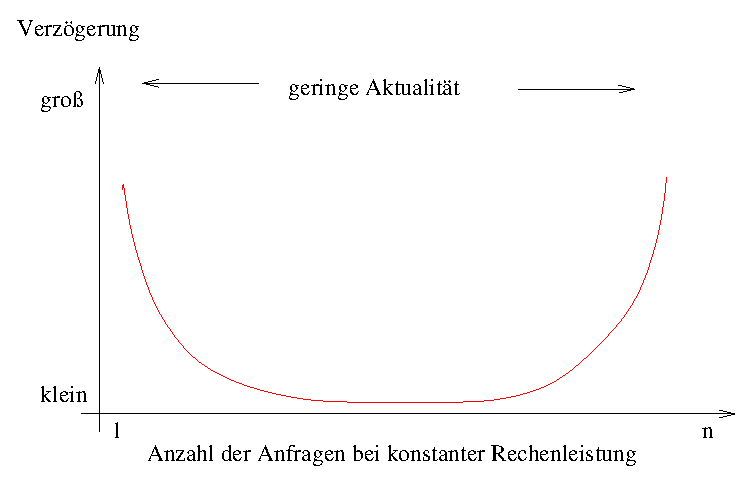
\includegraphics[bb=100 0 200 250,scale=0.9]{Zusammenhang_Pollingrate_Aktualitaetsgrad}
\end{picturehere}

Abbildung \ref{Abb:ZshgPollAkt} zeigt die Auswirkung der Polling-Rate (=1/Polling-Periode) auf den Aktualit�tsgrad der Informationen\footnote{Die Grafik soll
lediglich als schematische Illustration dienen, ein vermeintlicher exponentieller Zusammenhang wurde nicht beobachtet.}.
Solch ein Zusammenhang wurde mit Hilfe der weiter unten beschriebenen Simulationsumgebung validiert.

\paragraph{Dienstg�te:}
Wir ben�tigen eine Metrik,
um die Dienstg�te (``Quality of Service'', QoS, siehe auch \cite{BeFiMu:2006:QoSPubSub}) bestimmen zu k�nnen. Mit ihrer Hilfe ist f�r einen Benutzer nachvollziehbar, welche eventuellen Verbesserungen
ihm ein neues Verfahren gegen�ber dem bisherigen bietet. Daf�r definieren wir zwei Funktionen: $\Gamma_V$ gibt Aufschluss �ber den Verz�gerungsgrad
der RSS-Feeds, $\Gamma_A$ gibt Aufschluss �ber den Aktualit�tsgrad der RSS-Feeds.\\

Die zeitliche Verz�gerung eines RSS-Feeds wird in Abh�ngigkeit von der bevorzugten Polling-Periode in Prozent angegeben. $\Gamma_V$ ist also dann gr��er 0,
wenn ein Feed einen Benutzer nicht innerhalb der gew�nschten Zeit erreicht. $\Gamma_V$ bestimmt sich durch
\begin{equation}
  \Gamma_V:=\begin{cases}
    0& \text{wenn $(\varDelta pubDate-ppp) < 0$},\\
    \frac{100\cdot(\varDelta pubDate-ppp)}{ppp} & \text{sonst}.
  \end{cases}
\end{equation}

Dabei ist $\varDelta pubDate$ die Zeitspanne vom aktuellen Zeitpunkt bis zum am weitesten zur�ckliegenden Ereignis innerhalb des letzten RSS-Feeds.\\

$\Gamma_A$ bestimmt sich durch
\begin{equation}
  \Gamma_A:=\begin{cases}
    100& \text{wenn $(\varDelta pubDate-ppp) < 0$},\\
    \frac{100\cdot ppp}{\varDelta pubDate}& \text{sonst}.
  \end{cases}
\end{equation}

Beispielsweise bedeutet ein Aktualit�tsgrad eines Feeds von 50\%, dass der Feed erst nach der Zeit $2\cdot ppp$ einen Subscriber erreicht hat.

\paragraph{Wahl der Zufallsspanne:}
Es ist erforderlich, f�r die Berechnung von $\varDelta Z$ eine Gr��e heranzuziehen, welche sich den Gegebenheiten dynamisch anpasst.
$ppp$ ist eine feste Gr��e, bzw.
wird vom Subscriber willk�rlich gesetzt, sollte also nicht ohne weiteres herangezogen werden. Wir definieren die vom Subscriber nicht direkt beeinflussbare
Gr��e $cpp$, welche die aktuelle Polling-Periode bezeichnet, und setzen $\varDelta Z:=cpp$. Bezogen auf $t_x$ wird ein Subscriber also sp�testens nach Ablauf der
Zeit $cpp$ seine Anfrage an den RSS-Server stellen. Wie sich $cpp$ im Laufe der Zeit anpassen soll, werden wir im Abschnitt
\ref{css:staukontrolle_pubsubrss} schildern.

\paragraph{Initiale Belegung der aktuellen Polling-Periode:}
Zun�chst stellt sich die Frage, wie $cpp$ initial belegt werden soll, also bei Eintritt des Subscribers in das System.
Die Fragestellung nach einem initialen Timeout ist eine sehr grunds�tzliche, die auch bei anderen Protokollfamilien
eine Rolle spielt (z. B. bei TCP, siehe auch \cite{18216}). Die Problematik ist hier die folgende:
w�hlen wir eine sehr kurze Polling-Periode und treten gleichzeitig viele neue Subscriber dem System bei, so kann es eventuell zur �berlastung
des RSS-Servers kommen. W�hlen wir eine lange Periode, so erh�lt der betreffende Subscriber einen neuen Feed m�glicherweise erst sehr sp�t bzw. zu sp�t.
Wir haben jedoch einen konkreten Richtwert, den $ppp$, und wir w�hlen initial $cpp:=ppp$.
Es stellt sich die Frage, welcher alternative Wert angemessen w�re, da ``kurze Periode'' und ``lange Periode'' relative
Begriffe sind und sich auf die Leistungsf�higkeit des RSS-Servers und auf die Anzahl der Klienten im System beziehen. Beide sind aber bei Einstieg des Subscribers
in das System dem Subscriber noch nicht bekannt.
Jedoch hat der Subscriber ein konkretes Anliegen, n�mlich den Erhalt eines Feeds sp�testens nach der Zeit $ppp$. Also bildet der $ppp$  aus Sicht des Subscribers
den Richtwert. Wie durch die Wahl des $cpp$ auftretende Probleme reduziert werden k�nnen, werden wir in den
Abschnitten \ref{cs:ausbalancierung_der_polling-perioden} und \ref{cs:churn} n�her betrachten.\\

Es gilt also, die aktuelle Polling-Periode $cpp$ eines Klienten in Bezug auf $ppp$ minimal zu w�hlen, so dass die Ungleichung $0\leq\rho<1$ immer noch
erf�llt ist. Es bedarf einer Staukontrolle, die die Auslastung des Servers bestimmt und den Wert $cpp$ entsprechend anpasst.


\subsection{Staukontrolle}
Seitdem Computer-Netzwerke explosionsartig an Gr��e und Komplexit�t zugenommen haben, hat sich ein Problem verst�rkt bemerkbar gemacht: Datenstau.
Van Jacobson et. al. (\cite{jacobson88congestion}) schildert die Beobachtung, dass in der Zeit mitte der 1980er Jahre Internet-Gateways 10\% der
ankommenden Pakete aufgrund von Puffer�berl�ufen verwarfen. Laut seiner Aussage lag dabei das Problem nicht in den Protokollspezifikationen selbst, sondern
haupts�chlich in deren Implementierungen. TCP (Transmission Control Protocol) ist ein verbindungsorientiertes Transportprotokoll, mit dessen Hilfe der Gro�teil
des Netzwerkverkehrs vonstatten geht. Im Laufe der Zeit wurden in TCP Mechanismen eingebaut und verbessert, um Datenstau festzustellen und soweit wie m�glich
zu vermeiden.\\

Auf dem Gebiet der Regelungstechnik besch�ftigt man sich damit, wie eine Gr��e einen bestimmten vorgegebenen Wert erreichen und halten kann. Bei einer Regelung
finden Kontrollmechanismen
Anwendung, um Wertabweichungen festzustellen und auszugleichen.\\

Im Folgenden werden wir Techniken aus diesen Teilgebieten betrachten und diese auf ihre Tauglichkeit bez�glich der L�sung unseres beschriebenen Problems untersuchen.
Nicht alle der vorgestellten Techniken sind ohne weiteres auf unsere Problemstellung anwendbar, und wir werden eine L�sung entwickeln, die auf die konkrete
Problemstellung unter Ber�cksichtigung der gegebenen Umst�nde zurecht geschnitten ist.

\subsubsection{Staukontrolle bei TCP}
\label{css:tcp}
TCP (Transmission Control Protocol) ist ein verbindungsorientiertes �ber\-tra\-gungs\-pro\-to\-koll und kontrolliert die Daten�bertragung zwischen Sender und
Empf�nger der Endknoten. Dabei wird gew�hrleistet, dass jedes der einzelnen Datenpakete (die einen Datenstrom formen) den Empf�nger erreicht
und die Ordnung der Pakete
innerhalb des Datenstroms bestehen bleibt. Bei Datenstau handelt es sich um Verlust von Datenpaketen. Falls es zu Datenstau kommt, so tritt dieser immer an
Verbindungsknoten (einschliesslich des Empfangsknotens) auf und kann durch verschiedene Faktoren auf dem Weg zwischen Sender und Empf�nger hervorgerufen werden:
\begin{description}
  \item [Bandbreiten:]
    Unterschiedliche Bandbreiten auf dem Weg zwischen Sender und Empf�nger beeinflussen die �bertragungsgeschwindigkeit einer Verbindung
    nachteilig in der
    Form, dass die ``langsamste'' Leitung (also die mit der geringsten Bandbreite) die
    Gesamt-�bertragungsgeschwindigkeit vorgibt. Trifft eine schnelle Leitung auf eine langsame Leitung, so k�nnen die an der langsamen Leitung ankommenden
    Pakete nicht schnell genug weiter geleitet werden. An diesem Knoten kommt es zum Puffer�berlauf, �bersch�ssige Datenpakete gehen verloren.
  \item [Anzahl der Verbindungen:]
    An einem Knotenpunkt k�nnen mehrere Verbindungen zusammen kommen, die den Gesamt-Datenfluss an diesem Punkt erh�hen. Auch hier kann es zum Puffer�berlauf
    kommen, so dass �bersch�ssige Datenpakete verloren gehen.
\end{description}
Damit jedes ausgesandte Paket den Empf�nger erreicht, werden in TCP Best�tigungs-Nachrichten (Acknowledgements, im Folgenden kurz $acks$ genannt) versandt.
Erh�lt der Sender f�r ein gesendetes TCP-Datenpaket kein $ack$, so wird er das Datenpaket erneut senden. Ein wichtiger Bestandteil eines Datenpaketes ist
die Sequenznummer \cite{RFC2581}. Anhand der Sequenznummer kann ein $ack$ eindeutig einem versendeten Datenpaket zugeordnet werden. Innerhalb des $acks$ vermerkt
der Empf�nger ebenfalls, welches Datenpaket er als n�chstes erwartet \cite{RFC793}.
Um eine Staukontrolle zu erreichen wurden einige Algorithmen in TCP integriert (siehe \cite{jacobson88congestion}, wir halten uns dabei an die englischen
Bezeichnungen):
\begin{itemize}
  \item slow-start
  \item round-trip-time variance estimation
  \item exponential retransmit timer backoff
  \item more aggressive receiver ack policy
  \item dynamic window sizing on congestion
  \item Karn's clamped retransmit backoff
  \item fast retransmit
\end{itemize}

Dabei soll erreicht werden, dass die maximal m�gliche Bandbreite (begrenzt durch die minimale Bandbreite (``bottleneck'') auf dem Verbindungsweg, s. o.) voll
ausgenutzt wird, ohne
dass Pakete verloren gehen; es darf also kein Paket in das Netzwerk eingespeist werden, bevor ein altes Paket entfernt wurde (die Verbindung befindet sich dann im
``Equilibrium'', der Paketfluss ist ``conservative'' \cite{jacobson88congestion}). Im Folgenden wollen wir die wichtigsten der oben genannten Algorithmen
vorstellen. Eine genaue Herleitung und Analyse der Algorithmen geht jedoch �ber den Rahmen dieser Arbeit hinaus.
Wir verweisen auf die entsprechenden Quellen in den Literaturangaben.

\paragraph{more aggressive receiver ack policy:}
\footnote{Hier ist in \cite{jacobson88congestion} nicht eindeutig feststellbar,  worauf sich van Jacobson genau bezieht, da er diese Bezeichnung im weiteren Text
nicht mehr verwendet. Es erschien sinnvoll, die folgende im o. g. Text zu findende Erkl�rung diesem Thema zuzuordnen.}TCP
ist ``self-clocking'': da $acks$ erst nach Erhalt der entsprechenden Datenpakete versendet werden k�nnen, bestimmt die Rate der ankommenden $acks$ die
Rate, mit der weitere Datenpakete ausgesendet werden sollen. Die Senderate passt sich somit automatisch der Bandbreite an.

\paragraph{slow-start:}
Durch das ``self-clocking'' tritt nur beim Start des Datentransfers ein Problem auf, da
hier zun�chst eine feste Rate gew�hlt werden muss. Diese wird zu Beginn relativ niedrig gew�hlt, bzw. ein Staufenster ``congestion window'' ($cngw$) 
bestimmt die Anzahl der Pakete pro Sendevorgang. Bei Start des Transfers oder nach Paketverlust wird die Gr��e des Staufenster auf 1 gesetzt.
F�r jedes $ack$ wird das Staufenster um den Betrag 1 erh�ht. Begrenzt wird dessen Gr��e durch das ``advertised receiver window'',
welches vom Empf�nger festgelegt wird und angibt, wieviele Bytes maximal als n�chstes �bersendet werden sollen. Die Zunahme der Gr��e $w$ des
Staufensters geschieht in der Zeit
$rtt*log_2w$, wobei $rtt$ die ``round-trip-time'' des letzten versendeten Datenpaketes ist (Zeit zwischen Versenden eines Datenpaketes und Erhalt des
entsprechenden $acks$). Siehe dazu \cite{jacobson88congestion}, \cite{RFC2581}. 

\paragraph{round-trip-time variance estimation:}
$Acks$ k�nnen die Geschwindigkeit des Datenflusses steuern, doch was geschieht, wenn $acks$ aufgrund verloren gegangener Pakete ausbleiben? M�ssen sich
beispielsweise bei voll ausgenutzter Bandbreite pl�tzlich zwei Datenstr�me dieselbe Leitung teilen, kommt es bei gleichbleibender Datentransferrate mit Sicherheit zu
Paketverlusten und somit zu
ausbleibenden $acks$. Der Sender muss einen Timer unterhalten, bei dessen Ablauf das zuletzt gesendete Datenpaket erneut versendet wird (im Folgenden als
Retransmission bezeichnet). Paketverlust kann auch
durch Besch�digung der Daten w�hrend der �bermittlung auftreten. Nach van Jacobson \cite{jacobson88congestion} Liegt die Wahrscheinlichkeit daf�r aber weit
unter 1\%. Daher lassen Timeouts bei gut eingestellten Timern mit sicherer Gewissheit auf Paketverluste schlie�en \footnote{Zur Problematik
bei Timern siehe \ref{css:timer}}. Diese Timeouts werden pro Verbindung dynamisch berechnet; im Folgenden bezeichnet $rto$ das ``retransmission timeout''-Intervall,
also die Zeitdifferenz bis zum n�chsten Aussenden eines Datenpaketes. Entsprechend der TCP-Spezifikation
berechnet sich (siehe \cite{18216}):
\[rto=min(UBound, max(LBound, \beta * srtt))\]
$\beta$ ist dabei ein empirisch ermittelter Varianz-Faktor, $UBound$ und $LBound$ sind untere und
obere Schranke f�r den $rto$. $srtt$ ist die ``smoothed roundtrip time'' und wird wie folgt ermittelt:
\[srtt= \alpha * srtt+ (1 - \alpha) * rtt\] 
$\alpha$ ist ein ebenfalls empirisch ermittelter Gl�ttungsfaktor (``smoothing factor''). Empfohlene Werte sind f�r $\alpha:$ $0.8 \sim 0.9$ und f�r $\beta:$
$1.3 \sim 2$ \cite{18216}.\\
Laut van Jacobson \cite{jacobson88congestion} liegt hierin folgende Problematik: $\beta$ kann sich h�chstens an eine bis zu 30\% gesteigerte Last anpassen. Aber die
Varianz des Wertes $rtt$ steigert sich rapide mit ansteigender Last. Bei
Laststeigerung �ber die 30\%-Marke hinaus kommt es zu versp�teten $acks$. Der jeweilige abgelaufene Timer bewirkt eine Retransmission des entsprechenden
Datenpaketes, was zu unn�tiger Mehrarbeit des Netzwerkes und zu Bandbreitenverschwendung f�hrt. Daher wird $\beta$ ebenfalls dynamisch berechnet.
Eine Berechnungsmethode findet sich in \cite{jacobson88congestion}.

\paragraph{exponential retransmit timer backoff:}
Um den Datenstau durch mehrfach ausgesandte Pakete nicht noch zu vermehren, muss sich der $rto$ stetig vergr��ern.
Van Jacobson \cite{jacobson88congestion} stellt heraus, dass nur exponentielles Wachstum des $rto$ Erfolg verspricht.
Daher wird nach jedem erneuten Aussenden eines nicht best�tigten Datenpaketes der $rto$ verdoppelt.

\paragraph{dynamic window sizing on congestion:}
Ein Vergr��ern des $rto$ verhindert nur einen zus�tzlichen Datenstau durch erneut ausgesandte Datenpakete. Damit auch die im Anschluss daran neu
ausgesandten Pakete nicht wieder zum Anstieg des Datenstaus f�hren, wird ebenfalls die Gr��e der Staufenster $cwnd$ halbiert (exponentielle Abnahme).
Ausbleibende oder verz�gerte $acks$ geben nur Auskunft �ber auftretenden Datenstau. Sie k�nnen nicht anzeigen, ob die volle Bandbreite einer Verbindung auch wirklich
ausgenutzt wird. Daher sollte die Gr��e der Staufenster nach einem bestimmten Schema angehoben werden. Die Anpassung von $cwnd$ geschieht nach folgendem Prinzip:
\begin{itemize}
  \item Nach jedem Timeout wird $cwnd$ halbiert.
  \item Nach jedem $ack$ f�r neue Daten wird $cwnd$ um $1/cwnd$ erh�ht.
  \item Beim Senden wird das Minimum and Daten von $cwnd$ und dem ``receivers advertised window'' gesendet.
\end{itemize}

Dieser Algorithmus tr�gt zur Stauvermeidung (``congestion avoidance'') bei und besteht parallel zum ``slow-start''-Algorithmus. Van Jacobson gibt in
\cite{jacobson88congestion} ein Auswahlkriterium an, nachdem zustandsabh�ngig zwischen beiden Algorithmen ausgew�hlt wird.

\paragraph{Karn's clamped retransmit backoff:}
Sequenznummern erm�glichen die Zuordnung eines $acks$ zu dem entsprechenden Datenpaket. Kommt es aufgrund von Timeouts zu Retransmissionen
desselben Datenpaketes, so tritt ein Problem auf, welches Karn und Partridge in \cite{Karn1991} als ``retransmission ambiguity'' bezeichnen:
es kann nicht festgestellt werden, auf welche Aussendung desselben Datenpaketes sich das $ack$ bezieht. Damit ist nicht klar, anhand welches Paketes
sich der $rtt$ bestimmen soll, er wird in jedem Falle nicht verl�sslich sein. Verschiedene Protokollimplementationen behandeln dieses Problem
auf unterschiedliche Weise: teils wird die am l�ngsten zur�ckliegende Aussendung als Grundlage zur Berechnung herangezogen, teils die am k�rzesten zur�ckliegende
Aussendung.
Wird die am l�ngsten zur�ck liegende Aussendung  gew�hlt, so k�nnen der $rtt$, damit der $srtt$ und letztlich der $rto$ unverh�ltnism��ig in die H�he schie�en.
In vielen F�llen ist die nachteilige Wirkung nicht besonders gro�, da aufgrund des Datenstaus eine Drosselung der Datentransferrate erw�nscht ist.
Kommt es aufgrund anderer Ursachen zu Paketverlusten (z. B. bei verlustreichen Leitungen durch St�rsignale), so tritt das Gegenteil des gew�nschten Verhaltens
ein: der $srtt$ sinkt auf ein sehr niedriges Niveau, obwohl sich in diesem Falle die Datentransferrate erh�hen sollte.
Wird die am k�rzesten zur�ckliegende Aussendung herangezogen, so ist die Wahrscheinlichkeit laut Karn sehr gro�, dass die Zeitfolge zwischen dieser Sendung und dem
ankommenden $ack$ sehr kurz ist, obwohl sich das $ack$ auf eine weiter zur�ckliegende Sendung bezieht. Dies f�hrt zu einer drastischen Reduzierung des $srtt$,
was �berfl�ssige Retransmissionen und damit eine zus�tzliche Verschwendung der Bandbreite zur Folge hat (\cite{Karn1991},\cite{Jain1986}). Andere Implementationen
lassen die $rtt$ bei Retransmissionen au�er acht. Dies geht gut, solange der $rto$ nicht schneller ansteigt, als der Algorithmus sich adaptieren kann. Ist $\beta$
gut gew�hlt, so ist die M�glichkeit daf�r sehr gering. Tritt dieser Fall dennoch ein, so kommt es (wie im letztgenannten Fall) zu �berfl�ssigen Retransmissionen.\\

Um diesem Problem zu begegnen, schl�gt Karn folgenden Algorithmus vor \cite{Karn1991}:\\
Grunds�tzlich wird der $rto$ nach einem Timeout vergr��ert (``back-off'').
Erreicht ein $ack$ den Sender nach einer Retransmission eines Datenpaketes, so wird keine Neuberechnung des $rtt$ und $srtt$ vorgenommen. Daf�r wird der neu
ermittelte (``backed-off'') $rto$ als Grundlage f�r die n�chste Retransmission bzw. f�r die Aussendung des n�chsten Datenpaketes herangezogen. Nur wenn ein $ack$
den Sender ohne vorausgehende Retransmission erreicht, wird der $rto$ mit Hilfe des nun neu berechneten $srtt$ ermittelt.\\
Die Wahl des neuen $rto$ im Falle einer Retransmission muss laut Karn so erfolgen, dass der $rto$ gr��er ist als die tats�chliche Roundtrip-Time. Typischerweise
geschieht die Steigerung des $rto$ exponentiell (entsprechend des ``exponential retransmit timer backoff'', s. o.).

\paragraph{fast retransmit:}
Erreichen den Sender vier identische $acks$ in Folge, so wird der Sender das vom Empf�nger erwartete Datenpaket sofort aussenden, ohne auf das
Ablaufen des Retransmissionstimers zu warten. ``Slow-start'' wird so lange ausgesetzt, bis ein anderes, nicht zu den vorherigen identisches $ack$ den Sender
erreicht  (\cite{RFC2581}). Die identischen $acks$ lassen sowohl darauf schlie�en, dass ein Datenpaket verloren gegangen ist, als auch, dass andere Datenpakete den
Empf�nger h�chstwahrscheinlich erreichen, da die identischen $acks$ sonst ausgeblieben w�ren. Die den identischen $acks$ zugrundeliegenden Datenpakete beeinflussen
das Datenaufkommen nicht mehr, da diese schon die Empf�nger-Queue erreicht haben. Daher geht man davon aus, dass das erneute, schnelle Senden des fehlenden
Datenpaketes das Netz nicht wesentlich im Negativen beeinflusst. ``Fast retransmit'' sollte, muss aber nicht von einer konkreten TCP-Implementation unterst�tzt
werden.\\

Zus�tzliche Erweiterungen zum TCP in Hinsicht auf hohe Performanz finden sich in \cite{jacobson93tcp}.

\paragraph{Bezug zur Zielsetzung:}
Wie zu Beginn des Abschnittes gesagt, geht es darum, die Auslastung der Server-Queue stabil zu halten, bzw. daf�r zu sorgen,
dass die Ungleichung $0\leq\rho<1$ erf�llt
ist. Zeigen wir zun�chst die Parallelen zwischen unserem Kommunikationsmodell und der Ebene, auf der TCP Anwendung findet: bei unserem Kommunikationsmodell
befinden sich die kommunizierenden Parteien (RSS-Server, Subscriber) ebenfalls an Endknoten. Befindet sich der RSS-Server unter starker Last, so wird seine
Antwort (die �bermittlung des RSS-Feeds) l�nger auf sich warten lassen, als unter geringerer Last. Die $rtt$ zwischen Anfrage und dem vom RSS-Server �bermittelten
Feed (entsprechend einem $ack$) l�sst in gewissem Rahmen auf die Auslastung des Servers schlie�en. Auch in unserem Fall kann die Antwortzeit durch
ein starke Netzbelastung und dadurch verursachte
lange �bertragungszeiten negativ beeinflusst sein. Dies w�rde eventuell unser Ergebnis verf�lschen, da wir nur an der St�rke der Serverlast interessiert sind,
die Netzbelastung spielt f�r uns keine Rolle. Um Teill�sungen zu finden, wollen wir aber zun�chst von den Nachrichtenlaufzeiten abstrahieren. Auch in unserem
Falle muss der Subscriber, sollte die Server-Antwort ausfallen, seine Anfrage erneut senden. Daf�r sollte er ebenfalls einen Timer mit laufen lassen. Wie bei
TCP sollte sich der $rto$ stetig vergr��ern, um die Serverbelastung nicht noch zu steigern. Erreicht die Server-Antwort den Subscriber
lediglich versp�tet, nach dem die Anfrage bereits wiederholt gesendet wurde, kommt es hier in jedem Falle zum Problem der ``retransmission ambiguity'': der
Subscriber kann nicht zuordnen, auf welche Anfrage sich die Antwort bezieht,
da unser Ansatz keine Sequenznummern zul�sst. In diesem Sinne gibt es bei unserem Ansatz keinen Unterschied zwischen regul�ren Anfragen und Retransmissionen von
Anfragen, da sich der Informationsgehalt der Anfragen grunds�tzlich nicht unterscheidet. Ob wir an dieser Stelle Karns L�sung favorisieren oder eine andere L�sung
w�hlen, werden wir im Abschnitt \ref{css:staukontrolle_pubsubrss} er�rtern.

\subsubsection{Anwendung eines Regelkreises}
Die Aufgabe einer Regelung besteht darin, bestimmte Gr��en (Temperatur, Spannung, etc.) auf einen
vorgeschriebenen Wert zu bringen und diesen entgegen allen St�reinfl�ssen konstant zu halten (\cite{Bernstein1998}). Bei der Regelung unterscheidet man zwischen
verschiedenen Gr��en, die zusammen einen Regelkreis bilden: 
\begin{description}
  \item [Regelgr��e $x$] oder auch der Istwert: Gr��e, welche konstant gehalten werden soll und zu diesem Zweck erfasst wird
  \item [F�hrungsgr��e $w$] oder auch Sollwert: vorgegebener Wert, auf den die Regelgr��e eingestellt werden soll
  \item [St�rgr��e $z:$] Gr��e, die die Regelgr��e in unerw�nschter Weise beeinflusst
  \item [Regeldifferenz $x_d:$] Differenz zwischen F�hrungs- und Regelgr��e $x_d=w-x$
  \item [Stellgr��e $y:$] Gr��e, durch welche die Regelgr��e in erw�nschter Weise beeinflusst wird
\end{description}

\begin{picturehere}{1}{4}{Regelkreis}{Abb:Regelkreis}
 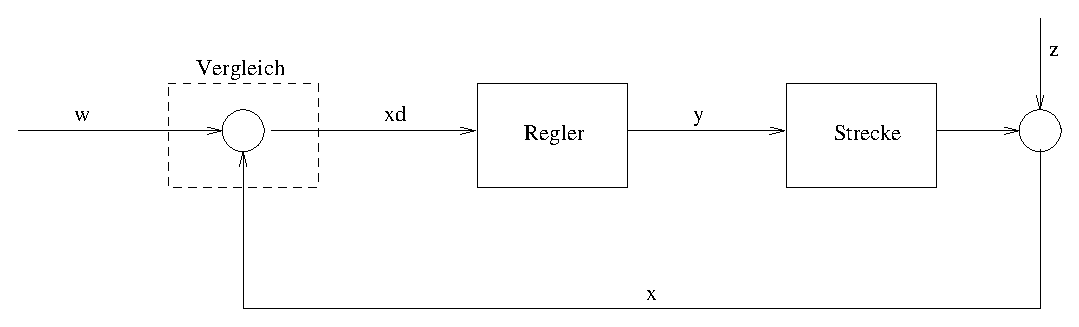
\includegraphics[bb=180 0 682 141,scale=0.75]{Regelkreis}
\end{picturehere}

%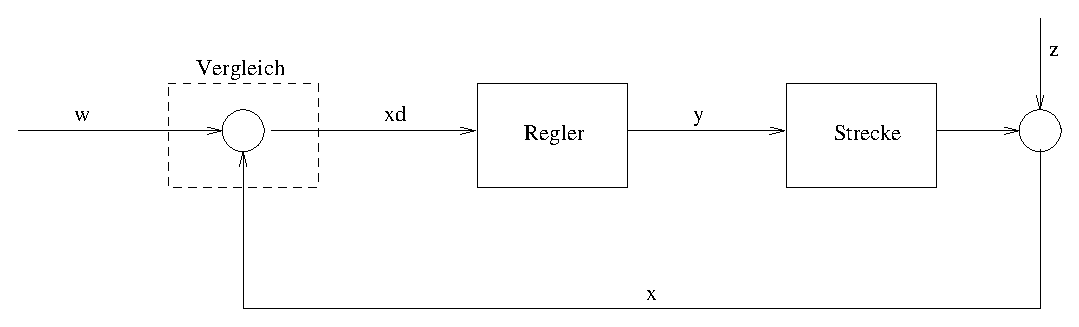
\includegraphics[scale=0.75]{Regelkreis.pstex}

Bild \ref{Abb:Regelkreis} zeigt das vereinfachte Schema eines Regelkreises. Die Regelung basiert auf R�ckkopplung. Bewirkt der Einfluss der St�rgr��e eine Abweichung
der Regelgr��e von der F�hrungsgr��e, so ergibt die Regeldifferenz �ber einen Regler eine Stellgr��e, die entgegengesetzt zur St�rgr��e auf die Regelgr��e einwirkt.
Ziel dabei ist es, die Regeldifferenz auf Null zu bringen.

Die Wahl eines geeigneten Reglers h�ngt stark von der Regelstrecke ab. Die Regelstrecke bezeichnet die zu regelnde Anlage oder den zu regelnden Proze�. Wichtig zu
wissen ist, wie die Regelstrecke auf �nderung der Einflussgr��en reagiert. Nach \cite{Bernstein1998} kann man die Regelstrecken grob durch folgende Merkmale 
unterscheiden:
\begin{itemize}
  \item Regelstrecken mit und ohne Ausgleich
  \item Regelstrecken mit und ohne Totzeiten bzw. Zeitglieder
  \item lineare oder nichtlineare Regelstrecken
\end{itemize}

Bei Regelstrecken mit Ausgleich erreicht die Ausgangs- bzw. Regelgr��e nach einer gewissen Zeit einen stabilen Zustand (Bsp. Raumtemperatur). Existiert kein
stabiler Zustand (Regelstrecke ohne Ausgleich), so �ndert sich bei konstanter Eingangs- bzw. Stellgr��e die Regelgr��e mit
konstanter Geschwindigkeit oder Beschleunigung (Bsp. F�llen eines Wasserbeh�lters). Totzeit bezeichnet eine Zeitverz�gerung, bis sich die �nderung der Stellgr��e
auf die Regelgr��e bemerkbar macht. Bei linearen Regelstrecken folgt die Regelgr��e der Stellgr��e proportional.

Meist liegt eine Kombination dieser Eigenschaften vor. Um die Stellgr��e entsprechend der Regeldifferenz anzupassen, wird ein Regler ben�tigt.

\paragraph{PID-Regler:}
Ein PID-Regler ist ein allgemeiner Reglertyp, der h�ufig f�r Regelungen Verwendung findet. Er ist eine Kombination aus einem P-, einem I- und einem D-Regler.
Ein P-Regler sorgt daf�r, dass (im station�ren Zustand) ein dem Eingangssignal proportionales Ausgangssignal geliefert wird (unter Zuhilfenahme eines
Verst�rkungsfaktors). Ein I-Regler summiert die Regeldifferenz �ber einen gewissen Zeitraum und f�hrt damit eine Integration aus. Je l�nger eine Regeldifferenz
besteht, desto gr��er wird die Stellgr��e. Ein D-Regler reagiert nur auf die �nderungsgeschwindigkeit der Regeldifferenz. Er liefert einen entsprechend starken,
kurzen positiven Impuls (ein reiner D-Regler hat in der Praxis keine Bedeutung).

Die allgemeine mathematische Gleichung f�r einen PID-Regler lautet wie folgt (siehe \cite{WBuettner1991}):
\[u(t)=K_R\left[\quad e(t) \quad + \quad \frac{1}{T_I}\int\limits_{0}^{t}e(\tau)d\tau \quad + \quad T_D\frac{de(t)}{dt} \quad \right]\]

Die einzelnen Gr��en sind:
\begin{description}
  \item [$u(t)$] Stellgr��e
  \item [$e(t)$] Regeldifferenz
  \item [$K_R$] Verst�rkungsfaktor
  \item [$T_I$] Integrationskonstante
  \item [$T_D$] Differentiationskonstante
\end{description}

Es werden nicht f�r alle Regelungen alle Anteile ben�tigt. Durch weglassen der entsprechenden Anteile erh�lt man die Regler P, PI bzw. PD. Reine P-Regler finden
nur Verwendung bei Regelstrecken linearen Verlaufs. Doch selbst hier zeigt sich, dass bei Regelabweichungen, die durch eine St�rgr��e hervorgerufen werden, die
St�rgr��e lediglich in ihrer Wirksamkeit gemindert werden kann. Eine vollst�ndige Beseitigung tritt nicht ein, da die Regelabweichung selbst notwendig ist, um eine
Verstellung des Stellgliedes vorzunehmen (\cite{Bernstein1998}). Mit einem I-Regler kann man die Regelabweichung sehr genau unterbinden, jedoch arbeitet dieser
relativ langsam und neigt zu Schwingungen. Die Vorteile beider Reglertypen vereint der PI-Regler. Reine D-Regler finden in der Praxis keine Verwendung, da sie bei
stabiler Regelgr��e nicht in den Regelvorgang eingreifen k�nnen. Die Kombination mit einem P-Regler (also ein PD-Regler) bewirkt ein schnelleres Anspringen der
Regelung bei pl�tzlicher Regelabweichung im Vergleich zu einem reinen P-Regler.\\

\paragraph{Bezug zur Zielsetzung:}
Wir k�nnen die Erf�llung der Ungleichung $0\leq\rho<1$ durch einen Regelkreis beschreiben. Die zu regelnde Gr��e ist dabei $\rho$. Die Stellgr��e
ist $cpp$. Aus Sicht eines Klienten
sind die $cpp$s der �brigen Klienten eine St�rgr��e, da ihre Ver�nderung die Auslastung des Servers beeinflusst. Bei der Regelstrecke handelt es
sich im allgemeinen um einen nicht-linearen Typ mit Ausgleich und Totzeit. Als Regler sollten wir daher einen PI-Regler verwenden. Eine differentiale Eigenschaft
wollen wir zun�chst au�er acht lassen, da diese nur zur Feinabstimmung beitr�gt.\\

Um $\rho$ messen zu k�nnen, muss der Regler einen direkten Zugriff auf die Werte $\lambda$ und $\bar x$ (s.o.) erhalten k�nnen.
Dies ist aber im allgemeinen, bzw. bei unserem
favorisierten Ansatz nicht m�glich, da nur der Server diese Werte ermitteln kann und diese entsprechend des Konzeptes nicht an die Klienten �bermittelt.
Ein Klient kann somit nur aufgrund anderer Indizien auf diese Werte r�ckschlie�en.
Das einzige Indiz ist das Antwortverhalten bzw. die Antwortzeit des Servers auf eine Anfrage des Klienten. Abstrahieren wir von den Nachrichtenlaufzeiten,
so l�sst eine lange Antwortzeit des Servers auf einen gewissen �berlastungsgrad schlie�en. Mit Hilfe der $rtt$ k�nnen wir somit die $cpp$ bestimmen, also
$cpp=f*rtt$, wobei $f$ ein beliebiger Faktor ist (proportionaler
Anteil des Reglers). Eine konstante Abtastrate w�re w�nschenswert, damit ein Regler zu jedem
Zeitpunkt die gleiche Reaktionszeit zeigen kann. Falls wir nur mit den regul�ren Anfragen nach RSS-Feeds zur Bestimmung der Server-Antwort arbeiten,
bewirkt eine Drosselung des $cpp$ ebenfalls eine Drosselung der Abtastrate.
Man k�nnte die Reaktionszeit des Servers anders ermitteln, z. B. durch konstantes Anpingen (z. B. mit Hilfe des Kommandos ``ping'').
Dies h�tte jedoch u. a. zur Folge, dass dadurch bei einer gro�en Anzahl Klienten im Overlay-Netzwerk ebenfalls
eine Server-�berlastung erreicht werden k�nnte. Die Beobachtung der zu regelnden Gr��e w�rde diese also gleichzeitig beeinflussen. Au�erdem erreicht ein Ping
nicht die Anwendungsschicht des Servers, eine �berlastung auf dieser Ebene bleibt eventuell unbemerkt. Des Weiteren kann es vorkommen,
dass eine Anfrage eines Klienten bei voller Queue vom Server verworfen wird. Eine Server-seitige Antwort wird in diesem Falle ausbleiben. Nach einem gewissen
Timeout muss also der Klient seine Anfrage erneut stellen. Ist dieses Timeout konstant und relativ klein, so kann dies ebenfalls zu einer Mehrbelastung des Servers
f�hren. Hierbei kommt das f�r den Regler erforderliche Ereignis (Server-Antwort) gar nicht zustande, somit kann eine Regelung �ber den Regler gar nicht in der
gew�nschten Weise stattfinden. Das Indiz f�r eine gesteigerte Server-Belastung ist hier also eine Negativ-Nachricht: das Ausbleiben der Server-Antwort. Um die
Mehrbelastung des Servers in diesem Fall einzud�mmen, k�nnen wir die Timeouts und somit die $ccp$ je nach Zeitdauer vergr��ern (integrativer Anteil,
vgl. Abschnitt \ref{css:tcp} TCP).\\

Es zeigt sich, dass das Konzept des PID-Reglers nur modifiziert anwendbar ist auf unsere Problemstellung.
Wie schon angedeutet, werden wir die Grundideen eines PID-Reglers in unserer hergeleiteten Methode wiederfinden.

\subsubsection{Staukontrolle bei Pub/Sub-RSS}
\label{css:staukontrolle_pubsubrss}



\subsection{Feeds und Timer}
\label{css:feeds_und_timer}
Bisher sind wir noch nicht weiter darauf eingegangen, welche ausl�senden Faktoren f�r das Setzen der Timer $RT$ und $RQT$ verantwortlich sind. Wir haben nur den
Timer $RT$ n�her betrachtet: ausl�sendes Ereignis ist die Aussendung eines Feed-Requests an den RSS-Server. Das Setzen des Timer-Intervalls $rto$ erfolgt wie im
vorherigen Abschnitt besprochen.\\

Bleibt zu bestimmen, wann und wie $RQT$ gesetzt wird. Erh�lt ein Subscriber einen RSS-Feed, so muss er bestimmen, wann der n�chste Feed-Request an den RSS-Server
gesendet werden soll. Dazu m�ssen wir einen erhaltenen Feed nach Aktualit�t und Herkunft unterscheiden. Erh�lt ein Subscriber einen neueren Feed von einem
Broker oder von einem RSS-Server, so
m�ssen $\varDelta Z$ und $t_x$, also $\varDelta ttr$, in Abh�ngigkeit von den enthaltenen Events entsprechend der in Abschnitt \ref{cs:der_grundlegende_algorithmus}
beschriebenen Methode neu bestimmt werden: f�r jeden RSS-Server, auf den sich ein neues Event bezieht, m�ssen diese Werte
neu berechnet und der entsprechende $RQT$ neu gesetzt werden. Erh�lt ein Subscriber dagegen einen Feed von einem Broker ohne neue Informationen,
so bleibt der laufende $RQT$ bestehen, denn dies ist genau der Fall, wo es in der Verantwortung des Subscribers liegt, in K�rze hinzukommende
Ereignisse abzufangen. Bei Erhalt eines Feeds von einem RSS-Server ohne neue Informationen muss $RQT$
neu gesetzt werden, denn es ist davon auszugehen, dass dem Feed ein Feed-Request aufgrund eines abgelaufenen $RQT$ vorausgegangen ist.
Dabei wird das $RQT$-Intervall auf $cpp$ gesetzt, $\varDelta Z$ wird nicht neu berechnet und $t_x$ wird auf $t_x:=t_0+cpp$ gesetzt.\\

Das ganze nochmal in an Java angelehnter Pseudonotation:

\begin{verbatim}

aktualisiereRQTdurchAltenBrokerFeed {
}

aktualisiereRQTdurchNeuenBrokerFeed {

    deltaTTR = berechneDeltaTTR(cpp);
    aktualisiereRQT(deltaTTR);

}

aktualisiereRQTdurchAltenServerFeed {

    aktualisiereRQT(cpp);

}

aktualisiereRQTdurchNeuenServerFeed {

    deltaTTR = berechneDeltaTTR(cpp);
    aktualisiereRQT(deltaTTR);

}


\end{verbatim}



\subsection{Ausbalancierung der Polling-Perioden}
\label{cs:ausbalancierung_der_polling-perioden}
Wie wir schon in Abschnitt \ref{cssp:ung_u_probl:dysbalance} auf Seite \pageref{cssp:ung_u_probl:dysbalance} beschrieben haben, kann es vorkommen, dass Subscriber
aufgrund von Dysbalancen der Polling-Perioden im System \glqq ausgesperrt\grqq{} werden: Subscriber, deren Polling-Perioden sehr niedrig sind, haben fast
ausschlie�lichen Zugriff auf den Server, w�hrend sich die Polling-Perioden der �brigen Subscriber stetig vergr��ern, da ihre Anfragen keinen Zugang zur Server-Queue
finden. Um diesem Problem beizukommen, m�ssen bei Dysbalancen im System Subscriber mit niedrigen Polling-Perioden diese erh�hen, w�hrend Subscriber mit hohen
Polling-Perioden Gelegenheit bekommen m�ssen, diese zu erniedrigen.\\

Um dieses Ziel zu erreichen, verwenden wir folgendes Verfahren: speist ein Subscriber einen RSS-Feed in das Notifikationssystem ein (er sendet den Feed an den
ihm zugewiesenen Broker), so �bermittelt er als zus�tzliches Attribut den von ihm gemessenen $artt$. Erh�lt ein Subscriber einen RSS-Feed vom Notifikationssystem,
so stellt sein neuer $artt$-Wert den Mittelwert aus seinem eigenen $artt$ und dem �bermitteltem $artt$ (im Folgenden nennen wir ihn $feed.artt$\footnote{Auch hier
gilt: pro Server muss ein feed.artt �bermittelt werden.}) dar, also:
\begin{equation}
  artt:=\frac{artt+feed.artt}{2}
\end{equation}
Es handelt sich dabei um ein kooperatives Modell: die gegenseitige Unterst�tzung der Subscriber wird vorausgesetzt, ein gemeinsames Ziel verlangt die Einschr�nkung
des Einzelnen.
\paragraph{Auswirkungen:}
Das Verfahren f�hrt dazu, dass Subscriber mit einer langen Polling-Periode, die einen Feed mit einem niedrigen $artt$ erhalten, ihre Polling-Periode senken,
allerdings nicht auf das Niveau des Subscribers, welcher den Feed ausgesandt hat. Somit wird eine zu schnelle �berlastung des Systems vermieden.
Im Gegenzug wird ein Subscriber mit einer gesenkten Polling-Periode schneller in den Genuss einer Server-Antwort kommen, so dass er ebenfalls einen Feed mit
seinem noch relativ hohen $artt$ in das Notifikationssystem einspeisen kann. Das f�hrt dazu, dass Subscriber mit einer niedrigen Polling-Periode diese bei Erhalt
jenes Feeds erh�hen.\\

Dies hat noch einen weiteren positiven Nebeneffekt: angenommen, alle Subscriber haben eine lange Polling-Periode aufgrund einer l�nger anhaltenden Server-�berlastung
eingestellt. Kommt es zu einer pl�tzlichen Reaktionsfreudigkeit des Servers, so wird der erste Subscriber, der diese feststellt, nicht nur seine Polling-Periode
entsprechend anpassen, sondern alle anderen Subscriber, die die Ansprechbarkeit des Servers nicht bemerkt haben, mitziehen. Ein pl�tzlicher �berm��iger Ansturm auf
den Server sollte aber ausbleiben, da die �brigen Subscriber ihre Polling-Perioden nicht drastisch, sondern nur allm�hlich senken. Die Subscriber, welche ihre
Polling-Periode drastisch gesenkt haben, werden gezwungen sein, ihre Polling-Periode wieder anzuheben. Dadurch erwarten wir eine homogenere Adaption der
Polling-Perioden an die Server-Auslastung.\\
Bei einer pl�tzlichen Server-�berlastung wird das jeder Subscriber schnell mitbekommen, weswegen sich in diesem Fall nicht viel �ndert.\\

Dadurch, dass der Wert $artt$ und nicht der Wert $cpp$ �bermittelt wird, kann jeder Subscriber seinen individuellen $cpp$-Wert entsprechend seiner Voreinstellungen
($ppp$) unabh�ngig der Voreinstellungen anderer Subscriber berechnen.\\

Die Wirksamkeit der ausbalancierenden Methode gegen�ber der nicht-ausbalancierenden Methode wird mit Hilfe der selbst entwickelten Simulationsumgebung gezeigt,
die Ergebnisse sind in Kapitel \ref{c:experimente} zusammengetragen.\\

Listen wir die Vorteile und m�glichen Nachteile dieser Methode auf:
\begin{itemize}
\item Vorteile
  \begin{itemize}
  \item Polling-Perioden werden ausbalanciert
  \item Bei unbemerkter Ver�nderung der Serverbelastung werden Subscriber mitgezogen
  \item Ansturm auf Server wird vermieden
  \end{itemize}
\item Nachteile
  \begin{itemize}
  \item Kooperatives Modell erfordert kooperatives Verhalten: spielen einige Subscriber nicht mit, wird die Idee des Systems untergraben. Das System kann nicht
    mehr in der gew�nschten Weise funktionieren.
  \end{itemize}
\end{itemize}

Das Verfahren erfordert auf der Ebene des Notifikationssystems neue Datenstrukturen, um den neu hinzugekommenen Wert $artt$ aufzunehmen\footnote{Wie bereits erw�hnt,
ist pro Server ein $artt$ notwendig.}. Folgende auf Java-Syntax beruhende Datenstrukturen sind denkbar:

\lstset{language=Java}
\begin{lstlisting}
class RichRSSFeed extends RSSFeed{

    LinkedList<RSSServerArtt> rssserver_artt;

}

\end{lstlisting}
\lstset{language=Java}
\begin{lstlisting}

class RSSServerArtt{

    RSSServer rssserver;
    long artt;

}

\end{lstlisting}

Nun muss bei jedem Erhalt eines RSS-Feeds der $cpp$ angepasst werden. Damit ein Subscriber zu jedem Zeitpunkt den derzeitigen Stand der gemessenen roundtrip-time
mitteilen kann, m�ssen nun jedesmal, wenn $RT$ abl�uft, $rtt:=rto$ gesetzt und $artt$ neu berechnet werden.
Daf�r ist es notwendig, die Methoden zur Aktualisierung des $RQT$ anzupassen.\\

Auch hierbei k�nnen gewisse Probleme und Seiteneffekte auftreten, die wir im Folgenden mitsamt L�sungen beschreiben.

\paragraph{$RQT$ verhindert Anfragen:}
Erh�lt ein Subscriber immer neue Feeds �ber das Notifikationssystem, bevor sein $RQT$ abgelaufen ist, so wird der $RQT$ st�ndig neu gesetzt, so dass
eine eigenm�chtige Aussendung eines Feed-Requests durch den Subscriber ausbleibt. Der Subscriber nimmt an der Versorgung des Notifikationssystems mit RSS-Feeds
nicht mehr aktiv Teil. Um hier Abhilfe zu schaffen, setzen wir den $RQT$ nur dann neu, wenn durch den neu gesetzten $RQT$ der anstehende Feed-Request fr�her
ausgesendet werden w�rde. Ansonsten kommt der neue
$cpp$ erst bei der n�chsten Runde in Betracht.

\paragraph{Beeinflussung des $cpp$:}
Was soll passieren, wenn ein Subscriber einen Feed �ber das Notifikationssystem erh�lt, w�hrend schon mehrfache Wiederholungen auftraten und der Subscriber
sich bei laufendem $RT$ gerade in der Messung der roundtrip-time befindet? Die Messung und die Wiederholungen sollten nat�rlich weiter laufen.
Nach unserem bisherigen Konzept hat der �bermittelte $feed.artt$ keinen Einfluss auf die zeitliche Abfolge wiederholter Anfragen.
Ist der Wert des �bermittelten $feed.artt$ gr��er als der $artt$-Wert des Empf�ngers zu Beginn der Messung, so ist dies ein akzeptables Verhalten,
denn der Wert des �bermittelten $feed.artt$ k�nnte aufgrund verloren gegangener Feed-Requests bestimmt worden sein und an der tats�chlichen roundtrip-time
vorbei gehen. Der empfangende
Subscriber hat noch die M�glichkeit, eine aussagekr�ftigere roundtrip-time zu bestimmen. Ist $feed.artt$ jedoch kleiner als der $artt$-Wert des Empf�ngers
zu Beginn der Messung, so w�re eine Einflussnahme von Vorteil, da der Wert des $feed.artt$ vermutlich aussagekr�ftiger ist. Denn entweder wurden weniger
Wiederholungen ben�tigt, um diesen zu
ermitteln, oder die Abtastrate (sprich die Rate der Feed-Requests) war h�her. Um dieses Verhalten zu erm�glichen, m�ssen wir einen neuen Wert definieren,
den $icpp$ (f�r initial-cpp), welcher als
Berechnungsgrundlage f�r $rto$ dienen soll und den $cpp$ in diesem Zusammenhang ersetzt. Bei jedem Setzen des $RQT$ wird $icpp$ auf
$icpp:=cpp$ gesetzt. Die Berechnung von $rto$ erfolgt dann nach jeder Aussendung einer Anfrage wie folgt:
\begin{equation}
rto:=2^i\cdot icpp
\end{equation}
Hierbei ist $i$ ebenfalls die Anzahl der Anfragen bzw. Verbindungsversuche.\\

W�hrend einer Messung der roundtrip-time kann der $cpp$ modifiziert werden, ohne dass dies einen Einfluss auf den $rto$ hat.
Da nach Abschluss der Messung $artt$ und somit $cpp$ neu berechnet werden, hat letztlich in diesem Fall die �bermittlung des $artt$ eines anderen Subscribers
keinen Einfluss auf den $artt$-Wert des empfangenden Subscribers. Im dem Fall jedoch, dass $feed.artt$ kleiner als der $artt$-Wert zu Beginn der Messung ist
(gilt dann, wenn $cpp<icpp$, da $cpp$ schon aufgrund des $feed.artt$-Wertes neu berechnet wurde), setzen wir $icpp:=cpp$.
W�rden wir diese Modifikation nicht vornehmen, h�tte in diesem Fall keine Ausbalancierung stattgefunden.\\

Unsere Algorithmen m�ssen wir also wie folgt modifizieren und vervollst�ndigen\footnote{Die Unterstriche kennzeichnen die neu hinzugekommenen Funktionen bzw.
Aufrufe.}:

\lstset{language=Java,emph={setze_icpp,berechne_mittleren_artt},emphstyle=\underbar}
\begin{lstlisting}

berechne_mittleren_artt(long feed.artt){

    setze_artt((feed.artt + artt) / 2);
    setze_cpp(artt);

    if ( cpp < icpp )
      setze_icpp(cpp);

}

\end{lstlisting}
\lstset{language=Java,emph={setze_icpp,berechne_mittleren_artt},emphstyle=\underbar}
\begin{lstlisting}

aktualisiere_RQT_durch_alten_Brokerfeed {

    berechne_mittleren_artt(long feed.artt);

    if ( RT_l�uft_nicht ){

      berechne_delta_ttr(cpp);
      if ( delta_ttr < RQT.Zeitdifferenz_bis_ablauf )
        setze_RQT(delta_ttr);

    }

}

\end{lstlisting}
\lstset{language=Java,emph={setze_icpp,berechne_mittleren_artt},emphstyle=\underbar}
\begin{lstlisting}

aktualisiere_RQT_durch_neuen_Brokerfeed {

    berechne_mittleren_artt(long feed.artt);

    berechne_delta_ttr(cpp);
    if ( delta_ttr < RQT.Zeitdifferenz_bis_ablauf )
      setze_RQT(delta_ttr);

}

\end{lstlisting}
\lstset{language=Java,emph={setze_icpp,berechne_mittleren_artt},emphstyle=\underbar}
\begin{lstlisting}

aktualisiere_RQT_durch_alten_Serverfeed {

    berechne_rtt();
    berechne_artt();
    setze_cpp(artt);
    setze_icpp(cpp);
    stoppe_RT();
    setze_rto_zur�ck();
    setze_RQT(cpp);

}

\end{lstlisting}
\lstset{language=Java,emph={setze_icpp,berechne_mittleren_artt},emphstyle=\underbar}
\begin{lstlisting}

aktualisiere_RQT_durch_neuen_Serverfeed {

    berechne_rtt();
    berechne_artt();
    setze_cpp(artt);
    setze_icpp(cpp);
    stoppe_RT();
    setze_rto_zur�ck();
    berechne_delta_ttr(cpp);
    setze_RQT(delta_ttr);

}

\end{lstlisting}

%%% Local Variables: 
%%% mode: latex
%%% TeX-master: "diplomarbeit"
%%% End: 

\subsection{Churn}
\label{cs:churn}
Ein Ph�nomen, welches bei Peer-To-Peer-Systemen h�ufig auftritt, ist \glqq Churn\grqq{}: das dynamische Zu- und Abwandern von Klienten bzw. Knoten. In
Peer-To-Peer-Systemen spielen die Klienten eine entscheidende Rolle. In fast allen diesen Systemen kommunizieren die Klienten direkt miteinander, um Daten
auszutauschen oder wichtige Informationen zu liefern (z. B. Dateien oder Routing-Informationen). Je nach Struktur des Peer-To-Peer-Netzes kann die pl�tzliche
Abwesenheit von beteiligten Knoten zu Beeintr�chtigungen oder gar Fehlfunktionen des Systems f�hren. W�hrend unstrukturierte Peer-To-Peer-Netze Churn zum Teil
gut verkraften, k�nnen strukturierte Peer-To-Peer-Netze (z. B. DHTs) mit Churn nicht anstandslos umgehen, bzw. sie ben�tigen spezielle Mechanismen, um den
Einfl�ssen von Churn entgegenzuwirken \cite{Stutzbach2004}.

\paragraph{Auswirkungen:}
Die Auswirkungen von Churn k�nnen verschiedenartig sein. So kann Churn beispielsweise bei BitTorrent dazu f�hren, dass sich Downloadzeiten verl�ngern, falls
Klienten das System verlassen, oder dass bestimmte Dateien nicht zugreifbar sind, falls ein Tracker ausf�llt. Bei DHT-basierten Netzen (neuere BitTorrent-Versionen
sind mittlerweile DHT-basiert) kann schon der
vor�ber\-gehen\-de Verlust eines Nachbarknotens zu Performanzeinbu�en f�hren (Effizienz ist ein Designziel bei DHT-basierten Peer-To-Peer-Systemen),
da der Ausgangsknoten gezwungen sein kann, suboptimale Routen zu w�hlen \cite{Rhea2004}.

\paragraph{Messung:}
Um Churn messen zu k�nnen, ist eine Metrik erforderlich, die �ber Zu- und Abwanderung Auskunft gibt. Es bietet sich an, die Zeit zwischen Betreten und Verlassen
des Systems durch einen Knoten zu messen. Beobachtungen haben gezeigt, dass sich die durchschnittlichen Zeiten zwischen einer Stunde und einigen Minuten bewegen
k�nnen \cite{Rhea2004}. Stutzbach und Rejaie \cite{Stutzbach2004} haben eine Reihe von Techniken entwickelt und in einem von ihnen entwickelten Tool
vereint, um das Gnutella-Netzwerk in relativ kurzer Zeit zu durchforsten und einen aktuellen Schnappschuss der Gnutella-Population zu
erhalten. Wie
Stutzbach und Rejaie feststellen, ist das Gnutella-Netzwerk ein sehr gro�es Peer-To-Peer-Netzwerk bestehend aus hunderttausenden von heterogenen und
geographisch verteilten Peers. Dar�ber hinaus wird jeder Client-Prozess direkt durch einen Benutzer gesteuert. Das hei�t, das \glqq Verhalten der User-Clients
repr�sentiert vollst�ndig Benutzer-gesteuerte Aspekte dynamischer Mitgliedschaften\grqq{} im System \cite{Stutzbach2004}. Ergebnisse einer solchen
Untersuchung k�nnen
damit f�r Peer-To-Peer-Systeme auf gleicher Basis herangezogen werden. Nach Stutzbach und Rejaie entspricht die Verteilung der Dauern, wie lange sich
Benutzer im System befinden, nicht, wie bisher angenommen, einer Poisson-Verteilung, sondern einer Exponentialverteilung.

\paragraph{Gegenma�nahmen:}
Um den Auswirkungen von Churn entgegen zu wirken, wurden einige Techniken in Abh�ngigkeit von der zugrunde liegenden Netzwerkstruktur entwickelt. Mit
Churn-Kompensation bei CMR-basierten Netzen (\glqq Concentric Multi-ring Overlay\grqq{}) besch�ftigen sich Wepiw\'e und Albayrak in \cite{Giscard2006},
bei DHT-basierten Netzen Rhea et al. in \cite{Rhea2004}. Ziel der beschriebenen Verfahren ist es, das Netzwerk in einem konsistenten Zustand zu
halten bzw. das Netzwerk schnell in einen solchen wieder zur�ckzuf�hren. Da diese Techniken keine Relevanz in bezug auf Churn bei \pubsubrss haben,
wollen wir hier nicht n�her darauf eingehen und verweisen auf die in der Literaturliste angegebenen Fachartikel.

\paragraph{Auswirkungen von Churn auf \pubsubrss:}
Verlassen einzelne Broker das Netzwerk, so liegen die Auswirkungen auf das Gesamtsystem nahe: der Verlust einzelner Broker
bedeutet ein Auseinanderfallen des Netzes in mehrere unabh�ngige Teilb�ume, falls das Broker-System baumartig aufgebaut ist oder falls genug Broker ausfallen.
W�hrend das Erfragen
von RSS-Feeds durch Subscriber und das Messen der roundtrip-times weiterhin vonstatten gehen kann,
k�nnen zwischen den Teilb�umen (\glqq Inseln\grqq{}) keine Nachrichten mehr
ausgetauscht werden. RSS-Feeds werden dadurch nicht mehr �ber das gesamte Overlay-Netzwerk verteilt.
Unter der Annahme, dass die Subscriber ihre Polling-Perioden optimal an die Server-Belastung angepasst haben und dieser an seiner
Belastungsgrenze arbeitet, kann ein Anheben der Polling-Perioden keinen Ausgleich schaffen. Je gr��er der Zerfall ist,
desto geringer wird folglich der Aktualit�tsgrad der RSS-Feeds in Inseln sein, in denen ein guter Aktualit�tsgrad durch den Erhalt
von RSS-Feeds �ber das Notifikationssystem zustande kam. Eine Anpassung der
Polling-Perioden der Subscriber an eine ver�nderte Serverbelastung wird einen l�ngeren Zeitraum beanspruchen, da weniger RSS-Feeds �ber das
Notifikationssystem verteilt werden und somit eine Ausbalancierung der Polling-Perioden in gerimgerem Ma�e erfolgen wird.\\
Welche Knoten in einem Netzwerk die Rolle der Broker �bernehmen, bleibt zun�chst offen. Ob Broker das System benutzergesteuert verlassen k�nnen, h�ngt ganz von der
jeweiligen Umsetzung des Systems ab. Denkbar sind beispielsweise dedizierte Knoten, welche dauerhaft online sind und kaum Ausfallerscheinungen aufweisen
(Supernodes bei Gnutella und KaZaA \cite{Aberer:P2P,KaZaA}). Daher tritt Churn auf Brokerebene in Abh�ngigkeit des jeweiligen Notifikationssystems auf. Um die Auswirkungen
von Churn auf dieser Ebene zu reduzieren, w�ren Rekonfigurationsverfahren auf Brokerebene notwendig. Cugola et al. besch�fftigen sich mit Rekonfigurationsalgorithmen
bei Publish-Subscribe-Systemen in \cite{cugola02towards,picco03efficient}.
Dies soll jedoch nicht Gegenstand dieser Arbeit sein und offen bleiben f�r zuk�nftige Entwicklungen.\\

Da in \pubsubrss Klienten nicht direkt miteinander kommunizieren, hat Churn weder Auswirkung auf die �bertragungsgeschwindigkeit von Daten noch auf die
Erreichbarkeit einzelner Daten (Feeds).\\
Verlassen Klienten das System, so hat das weniger Feed-Requests pro Zeiteinheit zur Folge, woraufhin die �brigen
Subscriber ihre Polling-Perioden verringern werden. Dies ist kein nachteiliger Effekt.\\
Beim Eintreten von Subscribern in das System stellen diese zun�chst ihren
$cpp$ auf den von ihnen gew�hlten $ppp$ ein. Erst im Laufe der Messung der roundtrip-times werden diese Subscriber ihren $cpp$ erh�hen. Bei einer hohen Anzahl von
neu in das System hinzukommenden Subscribern pro Zeiteinheit gibt es also eine erh�hte Rate an Feed-Requests. Dies bedeutet bei einer konstanten Churn-Rate eine
konstante Mehrbelastung des jeweiligen
RSS-Servers. Wir vermuten, dass, unabh�ngig davon, wie gut die Anpassung an die Serverbelastung vonstatten geht, die Mehrbelastung in diesem Fall mit der
bisherigen Methode schlecht kompensiert werden kann (siehe Abschnitt \ref{exp:churn_kompensation}).

\subsubsection{Churn-Kompensation bei \pubsubrss}
Um die negativen Auswirkungen von Churn bei \pubsubrss zu reduzieren, muss die Mehrbelastung des Servers durch neu hinzugekommene Subscriber so weit wie m�glich
vermieden werden. Eine L�sung kann aufgrund folgender �berlegung entwickelt werden: tritt ein Subscriber dem System bei, so existieren eventuell schon
gen�gend Subscriber, welche einen
aussagekr�ftigen $artt$ und $cpp$ berechnet haben. Der neu hinzugekommene Subscriber kann sich an diesen Richtwerten orientieren und muss seinen
individuellen $cpp$ nicht mit Hilfe seines $ppp$ als Ausgangswert berechnen. Es reicht aus, die Anzahl der Subscriber heranzuziehen, welche mit dem gleichen
lokalen Broker verbunden sind. Diese Information kann der lokale Broker ohne Schwierigkeiten liefern. Da nur $RichRSSFeeds$ einen Broker passieren (siehe Abschnitt
\ref{cs:ausbalancierung_der_polling-perioden}), kann dieser den enthaltenen $feed.artt$ eines Feeds zwischenspeichern. Betritt ein neuer Subscriber das System, so
kann der Broker diesem den aktuellen Feed mitsamt des zwischengespeicherten $artt$-Wertes �bermitteln. Der neue Subscriber w�hlt nun wie bisher seinen $cpp$ auf
Basis dieses $feed.artt$s. Dadurch steigen neue Subscriber bei der Messung der roundtrip-time bereits mit einer h�heren $cpp$ ein, wovon wir uns eine
Entlastung des RSS-Servers versprechen (siehe Abschnitt \ref{exp:churn_kompensation}).\\

Um dieses Verfahren zu realisieren, m�ssen wir eine zus�tzliche Datenstruktur und weitere Methoden zu unseren schon bestehenden hinzuf�gen:


\lstset{language=Java}
\begin{lstlisting}

public class InitialBrokerRSSFeed extends RSSFeed {

        zahl_lokaler_subscriber;
        artt;

}

speichere_initiale_brokerinformationen(InitialBrokerRSSFeed feed) {

        if ( feed.zahl_lokaler_subscriber < 2 )
          return;

        if ( feed.artt < 1 )
          return;

        setze_artt(feed.artt);
        setze_cpp(artt);
        setze_icpp(cpp);

        aktualisiere_RQT_durch_initialen_brokerfeed();

}

aktualisiere_RQT_durch_initialen_brokerfeed() {

        berechne_delta_ttr(cpp);
        setze_RQT(delta_ttr);

}

\end{lstlisting}


%%% Local Variables: 
%%% mode: latex
%%% TeX-master: "diplomarbeit"
%%% End: 


%%% Local Variables: 
%%% mode: latex
%%% TeX-master: "diplomarbeit"
%%% End: 


%%% Local Variables: 
%%% mode: latex
%%% TeX-master: "diplomarbeit"
%%% End: 
